% !TEX root = ../thesis.tex

%=========================================================
\chapter{SSN SET} 
\label{appendix:ssn-set}
%=========================================================

    %=========================================================
    \subsubsection*{TB Characterization}
    %=========================================================


        \singlefitfigure{ssn-set/tb-single}{
            bla
        }{fig:ssn-set:tb}

    %=========================================================
    \subsubsection*{Low-Conducting BJ}
    %=========================================================

        \begin{figure}[t]
            \centering
            \subfigure[bla]{\thesisplot{ssn-set/ssn-single}{iv}}
            \subfigure[bla]{\thesisplot{ssn-set/ssn-single}{didv}}
            \subfigure[bla]{\thesisplot{ssn-set/ssn-single}{dvdi}}
        \end{figure}

        \begin{figure}[t]
            \centering
            \subfigure[bla]{\thesisplot{ssn-set/sc-map/cal_iv}{main}}%
            \subfigure[bla]{\thesisplot{ssn-set/sc-map/cal_didv}{main}}%
            \subfigure[bla]{\thesisplot{ssn-set/sc-map/cal_dvdi}{main}}%
        \end{figure}

        \begin{wrapfigure}[11]{r}{1.6in}
            \captionsetup{format=plain}%
            \centering
            \vspace{-1.5em}
            % \thesisplot{ssn-set/}{dGdiff}
            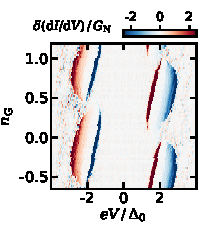
\includegraphics{ssn-set/dGdiff.pdf}
            \vspace{-.5em}
            \caption{
                    Linear fit to the low-voltage superconducting branch.
                }
        \end{wrapfigure}

    %=========================================================
    \subsubsection*{High-Conducting BJ}
    %=========================================================

        \begin{figure}[t]
            \centering
            \subfigure[bla]{\thesisplot{ssn-set/dcb-single}{iv}}%
            \subfigure[bla]{\thesisplot{ssn-set/dcb-single}{didv}}%
            \subfigure[bla]{\thesisplot{ssn-set/dcb-single}{dvdi}}%
        \end{figure}

        \begin{figure}[t]
            \centering
            \subfigure[bla]{\thesisplot{ssn-set/dcb-ssn-single}{iv}}%
            \subfigure[bla]{\thesisplot{ssn-set/dcb-ssn-single}{didv}}%
            \subfigure[bla]{\thesisplot{ssn-set/dcb-ssn-single}{dvdi}}%
        \end{figure}